\documentclass[12pt]{beamer} %slightly bigger font

% The preamble starts here.

\usetheme{default} % other themes are available; 'default' is fine, & simple

\setbeamertemplate{navigation symbols}{} %gets rid of navigation symbols
\setbeamertemplate{footline}{} %gets rid of bottom navigation bars
%\setbeamertemplate{footline}[page number]{} %use this if you want page numbers
\setbeamertemplate{itemize items}[circle] % gives you round bullet points (otherwise you get triangles)
\setlength\parskip{10pt} % adds white space between paragraphs

% From Ken Rice:
% - I will abuse the section/subsection/frame labeling system
% - I just use frame labels, not sections and subsections
% - Here is a `helper' functions to save typing, later
% This is an example of a 'macro'
\setbeamertemplate{frametitle continuation}[from second][ ]
\newcommand{\mystart}[1]{ \section{#1}\begin{frame}[allowframebreaks] \frametitle{#1} } 

% information for the title slide
\title{Introduction to \LaTeX } % title infomation
\subtitle{BIOST 561}
\author{Kelsey Grinde\footnote{Borrowing heavily from Katie Wilson and Ken Rice}}
%\institute{University of Washington Department of Biostatistics} %if you want to add your instution
\date{\today} 

% This concludes the preamble. 


% Now to start the document:
\begin{document}

% Title Slide
\begin{frame} %start a new slide
  \titlepage %puts the title information on a pretty title page
\end{frame} %end the slide; don't forget this

% Slide 2
\mystart{First things first...} %the \mystart command includes \begin{frame}
Is it \begin{huge} Lah-Tech \end{huge} or \begin{huge} Lay-Tech \end{huge} ?
\end{frame} % don't forget to end the slide!

% Slide 3
\mystart{What is \LaTeX ?}
  \begin{itemize} % a bulleted list
	\item ``A document preparation system for high-quality typsetting"
	\item It is \textit{not} a word processor like Microsoft Word 
  \end{itemize}
\end{frame}

% Slide 4
\mystart{Why use \LaTeX ?}
  \begin{itemize}% a bulleted list
	\item Formatting is clean, uniform, professional 
	\item Math formulas look great and they're easy to include
	\item Good for large documents (e.g., dissertations, textbooks)
	\item Handles citations easily 
  \end{itemize}

Why not use \LaTeX ?
	\begin{itemize}
		\item Have to remember lots of commands
		\item Need to compile before you can see the document
		\item Making comments, tracking edits not as straightforward
		\item Some applied journals prefer Word
	\end{itemize}
\end{frame}

% Slide 5
\mystart{How to get \LaTeX}

Everything you need is on Box. 

But, for your own computers:

	\begin{itemize}
	\item Get a \TeX \ \href{https://www.latex-project.org/get/}{distribution}
	\item Get a \TeX \ \href{https://en.wikipedia.org/wiki/Comparison_of_TeX_editors}{editor} (my favorite is texmaker)
	\item Or, compile using the department servers
	\end{itemize}
	
\end{frame}

\mystart{Basic Structure}

\begin{enumerate}
\item Specify type (``class") of document: \texttt{article}, \texttt{beamer}
\item (Optional preamble)
\item Begin document
\item (Insert your text here)
\item End document
\end{enumerate}

An example....

\end{frame}


% Example1
\begin{frame}[fragile]

Example 1:

\begin{verbatim}
\documentclass{article}
\begin{document}
This is a sentence.
\end{document}
\end{verbatim}
\end{frame}


% New slide
\mystart{Compiling}
  \begin{enumerate}
  \item Save your code as \texttt{filename.tex}
  \item Compile
  	\begin{itemize}
  	\item Open in \TeX \ editor, ``Build"/``Typeset"
  	\item Use department servers: \texttt{pdflatex filename.tex}
  	\item Errors displayed on console and in \texttt{.log} file
  	\end{itemize}
  \item Open \texttt{.pdf} (other files created, but you can ignore)
  \end{enumerate}
\end{frame}

% Example2
\begin{frame}[fragile]

Example 2:

\begin{verbatim}
\documentclass{article}
%Start of preamble
\title{Example Document}
\author{Kelsey] %there is an error here
\date{November 2, 2017}
%End of preamble
\begin{document}
\maketitle
This is a sentence.
\end{document}
\end{verbatim}
\end{frame}

\mystart{\LaTeX \ Commands}
\begin{itemize}
\item Start with a backslash, usually contain letters only
\item End with a space, number, or non-letter
\item Required parameters (if applicable) specified within \{ \} after command
\item Optional parameters (if applicable) specified within [ ] after command
\end{itemize}

Example: \texttt{\textbackslash maketitle}
\end{frame}

\mystart{Text Commands}

\begin{itemize}
\item \texttt{\textbackslash underline}: \underline{underline}
\item \texttt{\textbackslash textit}: \textit{italicize}
\item \texttt{\textbackslash textbf}: \textbf{bold}
\item \texttt{\textbackslash texttt}: \texttt{typewriter}
\item \texttt{\textbackslash\textbackslash}: line break
\item \texttt{\textbackslash}: add a \ space
\item \texttt{\textbackslash LaTeX}: writes \LaTeX
\item \texttt{\textbackslash clearpage}: inserts page break at current position
\item \texttt{\textbackslash par}: start new paragraph
\item \texttt{\textbackslash today}: today's date \today
\end{itemize}
\end{frame}

\mystart{Font Size}

\tiny{tiny} \scriptsize{scriptsize}
\footnotesize{footnotesize}
\small{small}
\normalsize{normalsize}
\large{large}
\Large{Large}
\LARGE{LARGE}
\huge{huge}
\Huge{Huge}

\end{frame}

\begin{frame}[fragile]{Special Characters}

Symbols with special meaning in \LaTeX :
\begin{verbatim}
# $ % ^ & _ { } ~ \
\end{verbatim}

Need to put backslash in front of them:
\begin{verbatim}
\# \$ \% \^ \& \_ \{ \} \~ \textbackslash
\end{verbatim}

\end{frame}

\mystart{Math Symbols}

Many built in commands:
\begin{itemize}
\item \texttt{\textbackslash beta}: $\beta$
\item \texttt{\textbackslash hat\{p\}}: $\hat{p}$
\item \texttt{\textbackslash sum\_\{i=1\}\^}\texttt{n}: $\sum_{i=1}^n$
\item \texttt{\textbackslash sim}: $\sim$
\item \texttt{\textbackslash approx}: $\approx$
\end{itemize}

\end{frame}

\mystart{Typing Math}

\begin{itemize}
\item Inline: $\hat\beta = \left( \mathbf{X}^T \mathbf{X} \right)^{-1}\mathbf{X}^T \mathbf{y}$
	\begin{itemize}
	\item \textbackslash (...\textbackslash )
	\item \$ ... \$
	\end{itemize}
\item Display mode: $$\hat\beta = \left( \mathbf{X}^T \mathbf{X} \right)^{-1}\mathbf{X}^T \mathbf{y}$$
	\begin{itemize}
	\item \$\$ ... \$\$
	\item \textbackslash [ ... \textbackslash ]
	\item \texttt{equation}, \texttt{eqnarray}, \texttt{align} environments
	\item Comparison here\footnote{\href{https://tex.stackexchange.com/questions/40492/what-are-the-differences-between-align-equation-and-displaymath}{https://tex.stackexchange.com/questions/40492/what-are-the-differences-between-align-equation-and-displaymath}}
	\end{itemize}
\end{itemize}

\end{frame}


% align example
\begin{frame}[fragile]

\begin{verbatim}
\begin{align}
E(\hat\beta) 
& = E \left[(X^\top X)^{-1} X^\top y \right] \\
& = (X^\top X)^{-1} X^\top E \left[ y \right] \\
& = (X^\top X)^{-1} X^\top X \beta \nonumber \\
& = \beta
\end{align}
\end{verbatim}

\begin{align}
E(\hat\beta) 
& = E \left[(X^\top X)^{-1} X^\top y \right] \\
& = (X^\top X)^{-1} X^\top E \left[ y \right] \\
& = (X^\top X)^{-1} X^\top X \beta \nonumber \\
& = \beta
\end{align}

\end{frame}

% matrix examples
\begin{frame}[fragile]

\begin{verbatim}
\[\left( \begin{array}{cc}
a & b \\
d & e \\
\end{array} \right) \]
\end{verbatim}

\[\left( \begin{array}{cc}
a & b \\
d & e \\
\end{array} \right) \]

\begin{verbatim}
\[\begin{bmatrix}
a & b \\
d & e \\
\end{bmatrix}\]
\end{verbatim}

\[\begin{bmatrix}
a & b \\
d & e \\
\end{bmatrix}\]

\end{frame}

% another array example
\begin{frame}[fragile]

\begin{verbatim}
\[ I(x<10) = \left\{ \begin{array}{ll}
1 & \mbox{if $x < 10$}; \\
0 & \mbox{if $x \geq 10$}. \end{array}\right. \]
\end{verbatim}

\[ I(x<10) = \left\{ \begin{array}{ll}
1 & \mbox{if $x < 10$}; \\
0 & \mbox{if $x \geq 10$}. \end{array}\right. \]

\end{frame}

% Environments
\mystart{\LaTeX \ Environments}

\begin{itemize}
\item Helpful for formatting entire blocks of text
\item Start with \texttt{\textbackslash begin} statement
\item End with \texttt{\textbackslash end} statement
\item Examples:
	\begin{itemize}
	\item array, bmatrix, align
	\item itemize, enumerate (bulleted, numbered lists)
	\item table, figure
	\end{itemize}
\end{itemize}
\end{frame}

\mystart{Tables}
\begin{itemize}
\item \texttt{tabular} environment
\item Specify column alignment (\underline{l}eft, \underline{c}enter, \underline{r}ight)
\item Separate columns with \&, separate rows with \textbackslash \textbackslash
\item Vertical lines with $|$, horizontal lines with \texttt{\textbackslash hline}
\item The \texttt{R} packages \texttt{xtable} and function \texttt{kable} in the \texttt{knitr} package can sometimes help
\end{itemize}

\pagebreak

\begin{center}
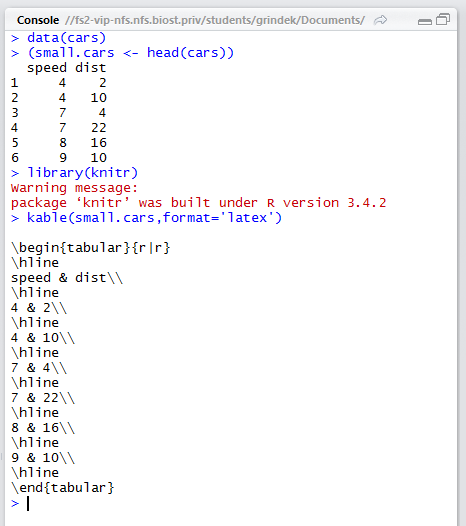
\includegraphics[height=0.9\textheight]{kableExample}
\end{center}

\end{frame}

% Table Example
\begin{frame}[fragile]{Tables}

\begin{verbatim}
\begin{tabular}{|r|cccrl|}
\hline
& & & \multicolumn{3}{c|}{Survival at 10 years} \\
& Total & Events & \% & \multicolumn{2}{c|}{95\% CI} \\
\hline
Group 1 & 12 & 11 & 90.9 & 75.4 & 100.0 \\
Group 2 & 11 & 7 & 66.7 & 44.7 & 99.5 \\
\hline
\end{tabular}
\end{verbatim}

\begin{tabular}{|r|cccrl|}
\hline
& & & \multicolumn{3}{c|}{Survival at 10 years} \\
& Total & Events & \% & \multicolumn{2}{c|}{95\% CI} \\
\hline
Group 1 & 12 & 11 & 90.9 & 75.4 & 100.0 \\
Group 2 & 11 & 7 & 66.7 & 44.7 & 99.5 \\
\hline
\end{tabular}

\end{frame}

% Figures
\mystart{Figures}
\begin{itemize}
\item Use the \texttt{graphicx} package
\item Lets you include pdf, png, jpeg, gif
\item Include captions with \texttt{\textbackslash caption}
\item Label for easy referencing with \texttt{\textbackslash label}
\item Cannot be broken over pages (tables, too), so considered to be a ``float"
	\begin{itemize}
	\item If it doesn't fit on current page, will be ``floated" to a later one
	\item Some control over this (e.g., \texttt{[h]} = here, \texttt{[t]} = top, \texttt{[h!]} = ignore other parameters that might prevent float from being placed here)
	\end{itemize}
\end{itemize}
\end{frame}

% Figure Example
\begin{frame}[fragile]{Figures}

\begin{verbatim}

\includegraphics[width=0.5\linewidth]{RooHalloween}
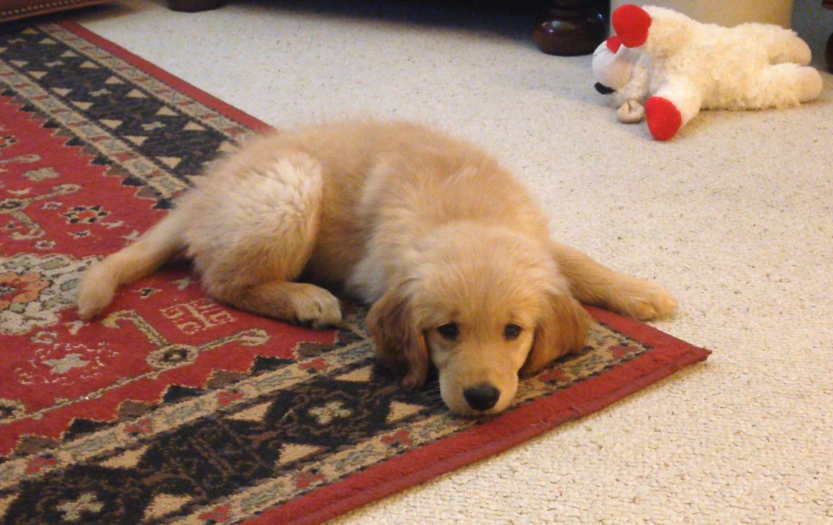
\includegraphics[scale=0.3, angle=90]{RooPuppy}
\end{verbatim}


\includegraphics[width=0.5\linewidth]{RooHalloween}
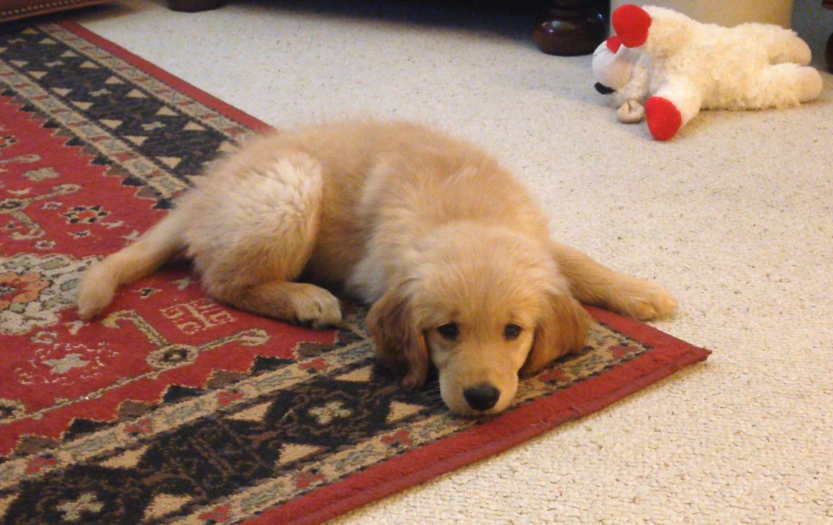
\includegraphics[scale=0.3, angle=90]{RooPuppy}

\end{frame}

%Floats example
\begin{frame}[fragile]

\begin{small}
\begin{verbatim}
My dog was a ``hot" dog for Halloween
(see Figure \ref{puppy})
\begin{figure}[h!]
\centering

\includegraphics[height=0.3\textheight]{RooHalloween}
\caption{Adorable puppy dressed as sriracha bottle.}
\label{puppy}
\end{figure}
\end{verbatim}
\end{small}

My dog was a ``hot" dog for Halloween
(see Figure \ref{puppy})
\begin{figure}[h!]
\centering

\includegraphics[height=0.3\textheight]{RooHalloween}
\caption{Adorable puppy dressed as sriracha bottle.}
\label{puppy}
\end{figure}

% can also do this referencing with tables, sections

\end{frame}

% Macros (defining your own commands)
\mystart{Macros}
\begin{itemize}
\item Define your own commands instead of typing the same thing over and over again
\item Specify in preamble
\item Or, store in another file (\texttt{preamble.tex}) and load this in with \texttt{\textbackslash include\{preamble.tex\}}
\end{itemize}

Example: \texttt{\textbackslash newcommand\{\textbackslash R\}\{\textbackslash mathbb\{R\}\}} will produce $\mathbb{R}$ by writing \texttt{\textbackslash R} rather than \texttt{\textbackslash mathbb\{R\}}
\end{frame}

% BibTeX
\mystart{Bib\TeX}
\begin{itemize}
\item Citation tool
\item Keep one file with information about all sources (\texttt{mybib.bib})
\item Easy to reference any source in that file, in whatever style is needed (e.g., APA)
\item To get information for \texttt{mybib.bib} file: Google Scholar $>$ Cite $>$ Bib\TeX
\end{itemize}

\end{frame}

% Example .bib file
\begin{frame}[fragile]{Bib\TeX}
My \texttt{mybib.bib} file contains the following entry:

\begin{verbatim}
@article{mckeague2015adaptive,
  title={An adaptive resampling test for detecting the presence of significant predictors},
  author={McKeague, Ian W and Qian, Min},
  journal={Journal of the American Statistical Association},
  volume={110},
  number={512},
  pages={1422--1433},
  year={2015},
  publisher={Taylor \& Francis}
}
\end{verbatim}

\end{frame}

\begin{frame}[fragile]{Bib\TeX}

Let's look at an example where we cite this article two different ways:

\begin{small}
\begin{verbatim}
\documentclass{article}
\usepackage{natbib}
\begin{document}
I thought \cite{mckeague2015adaptive} was very 
interesting. In fact, it was so interesting that I'm going 
to cite it two different ways \citep{mckeague2015adaptive}.
\bibliographystyle{plainnat}
\bibliography{mybib}
\end{document}
\end{verbatim}
\end{small}

\end{frame}


% Beamer (for making slides)
\mystart{Beamer}
\begin{itemize}
\item For making slides like these!
\item It's a document class: \texttt{\textbackslash documentclass\{beamer\}}
\item There are many different themes
	\begin{itemize}
	\item I'm using the default
	\item Others \href{http://deic.uab.es/~iblanes/beamer_gallery/index_by_theme.html}{here}
	\end{itemize}
\item Take a look at my slides (and corresponding \texttt{.tex} file) for example
\end{itemize}
\end{frame}



% Miscellaneous
\mystart{Miscellaneous}
\begin{itemize}
\item You can define your own class
	\begin{itemize}
	\item \texttt{\textbackslash documentclass\{myclass.cls\}}
	\item Or, use someone else's class file. I did this for my CV (you can find resume class files online)
	\item There's one for UW dissertations: \href{https://staff.washington.edu/fox/tex/uwthesis.shtml}{\texttt{uwthesis.cls}}
	\end{itemize}
\item You can use \LaTeX \ to make posters
\item Need help? Ask Google.
\item You can do nearly all of this in R Markdown
\end{itemize}

\end{frame}


\end{document} % don't forget this

